\section{XSS}
The objective of a XSS attack is to inject malicious js into the victim's page. The attacker uses vulnerabilities in the web application, not the web browser, to store this malicious scripts in the server, so that when the victim visits the webpage the js executes without the user's interaction. Malicious js can be very dangerous, as it can steal unprotected cookies, make requests in the user's behalf and modify the page's html to create phishing attacks, between many others. If an attacker can use the web app to execute js in another user's browser, the security of the site and it's users is severely compromised.
\subsection{Types of XSS}
\subsubsection{Persistent XSS}
In this attack, the malicious js is stored in the DB. The attacker can upload this js disguised in a comment of a post, a form, etc. The web app saves this code in the DB, and when the page is solicited by another user the code is inserted in the html unknowingly by the application.
\begin{figure}[htb]
	\begin{centering}
		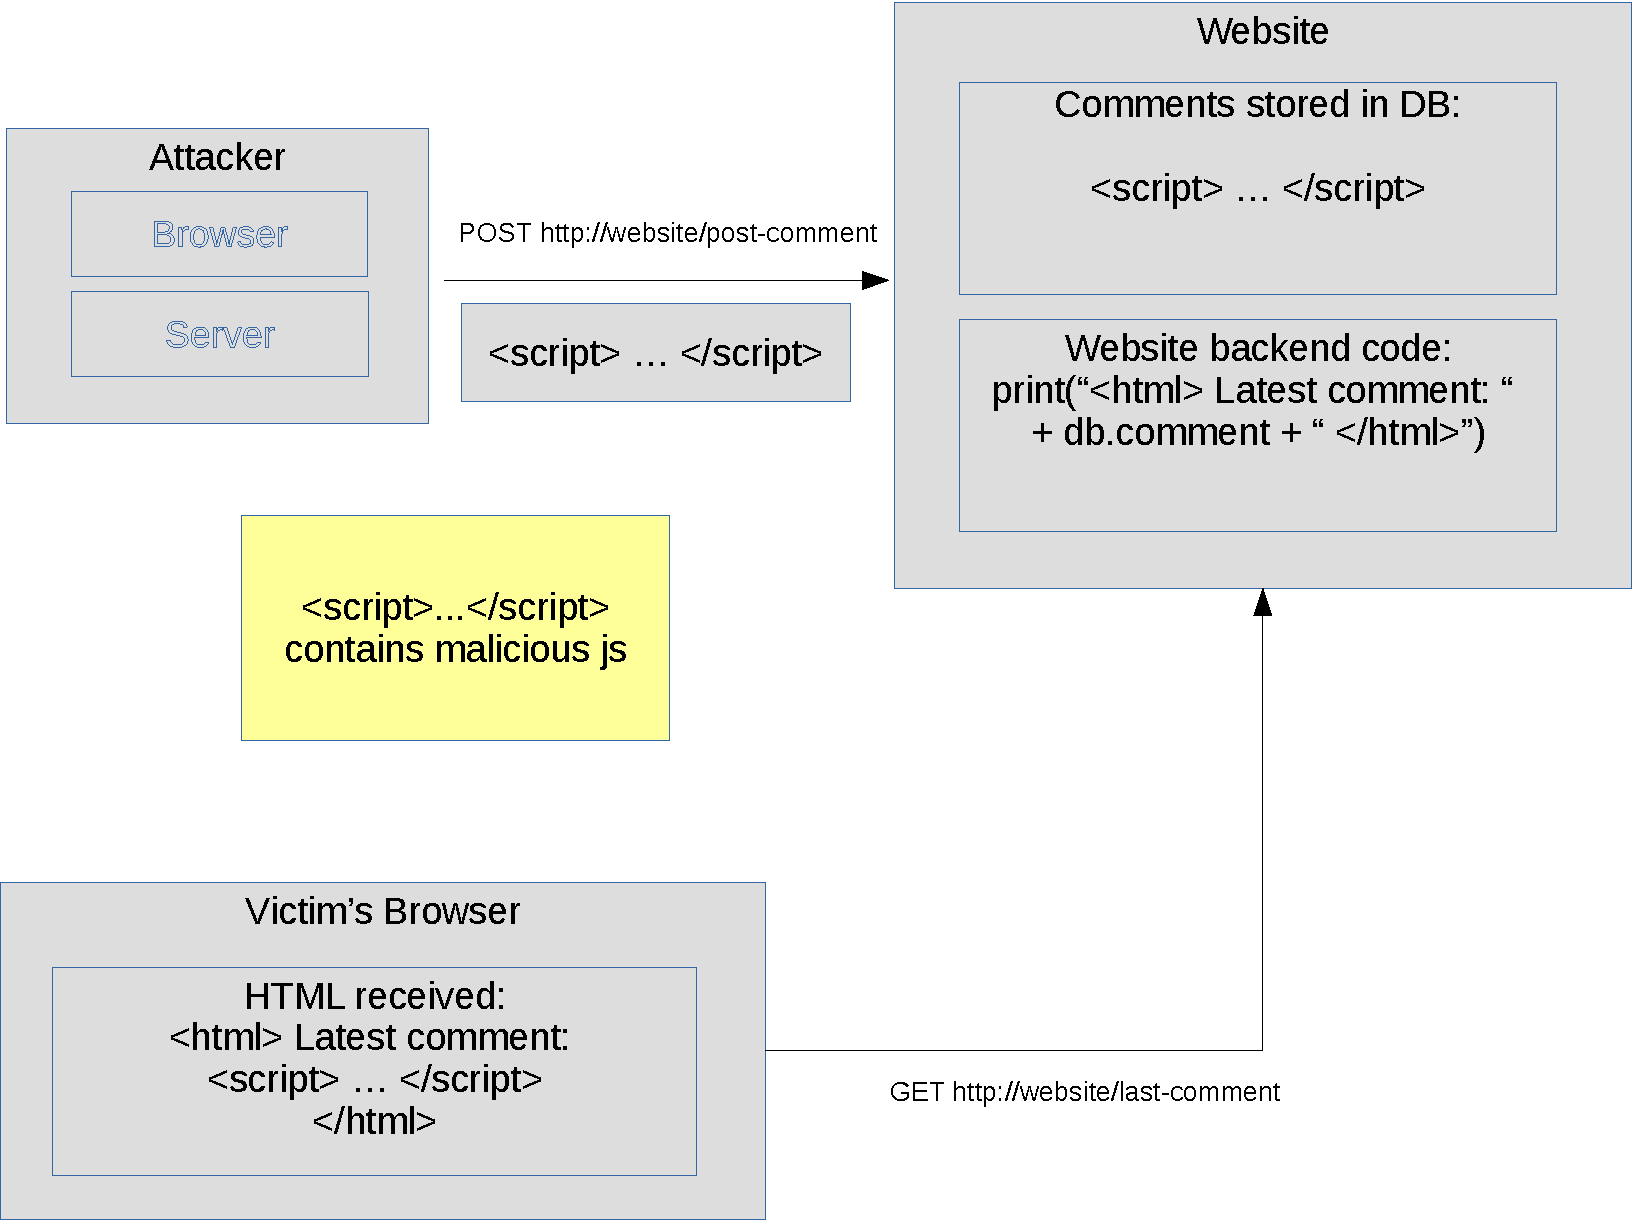
\includegraphics[width=0.7\columnwidth]{\securitydir/WebSec/figures/persistent-xss}
		\par\end{centering}
	\caption{\label{fig:ecb} Diagram of a stored XSS exploit.}
\end{figure}

\subsubsection{Reflected XSS}
The attacker needs to craft a malicious URL with js in it as a parameter. This is usually exploited passing a URL with a search query with the js as the paramater to search. The attacker then tricks the victim to open the link, generating a GET request and returning HTML page with the query inserted in it. https://excess-xss.com/reflected-xss.png
\begin{figure}[htb]
	\begin{centering}
		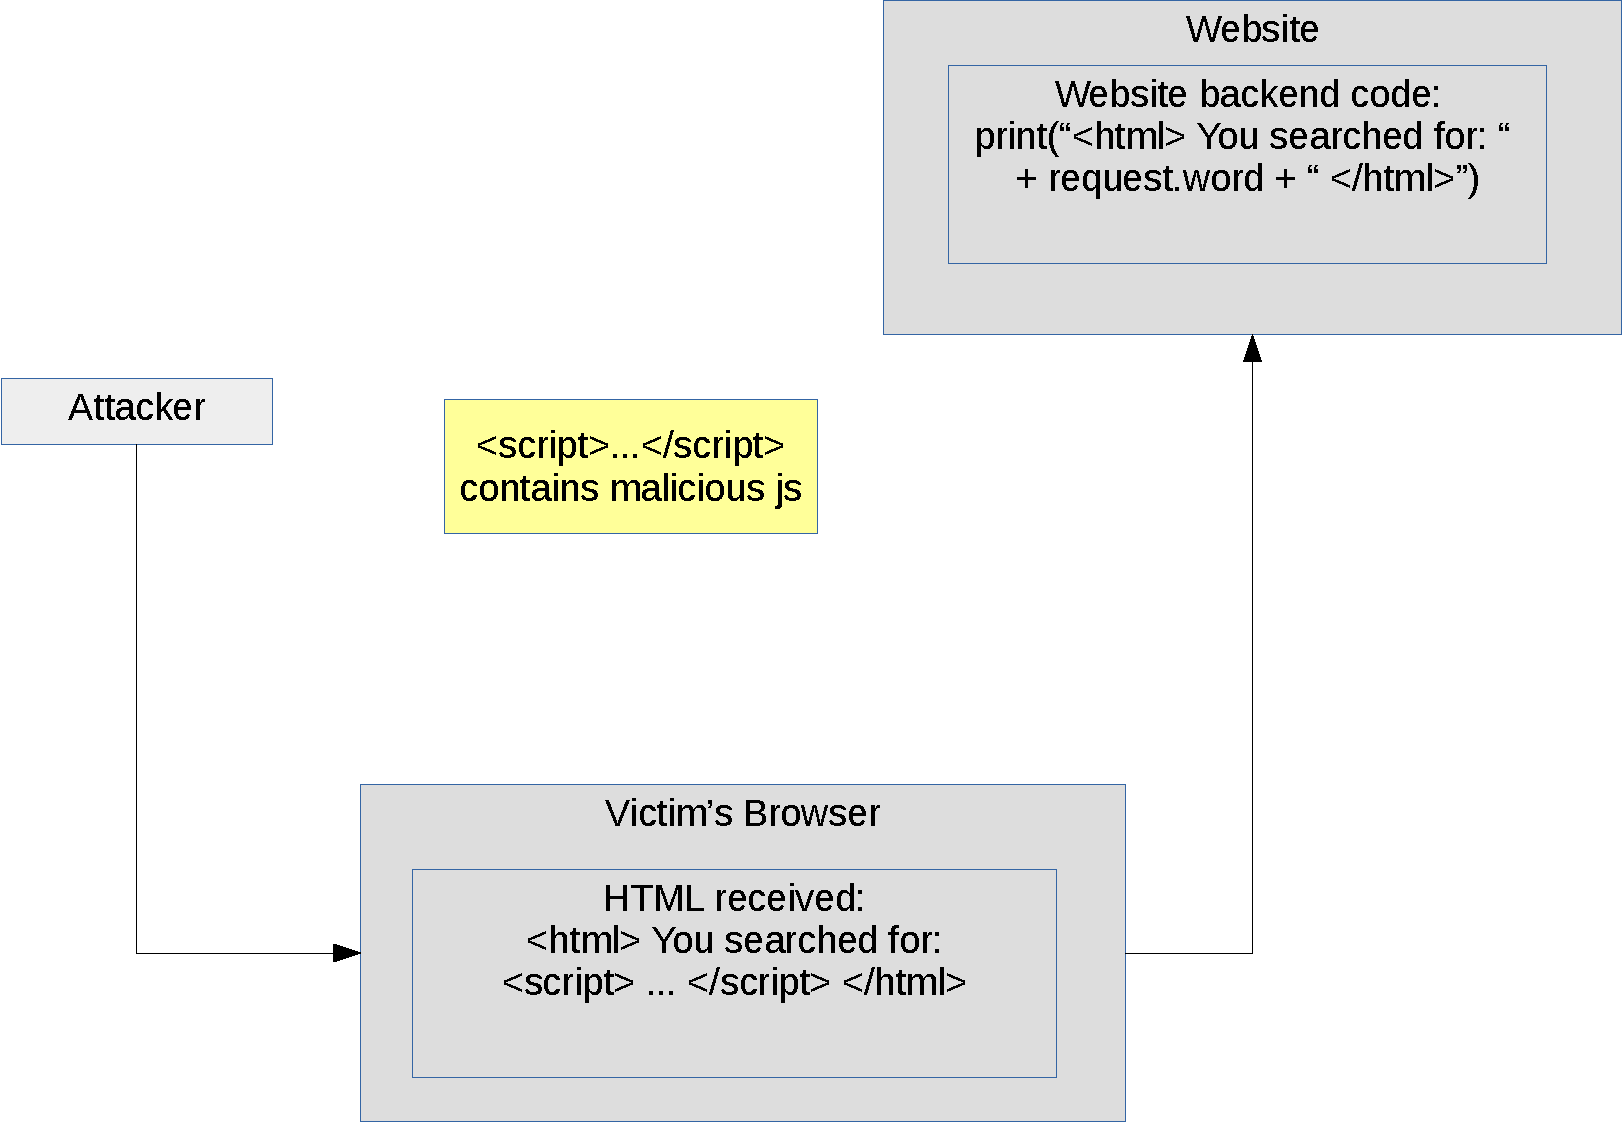
\includegraphics[width=0.7\columnwidth]{\securitydir/WebSec/figures/reflected-xss}
		\par\end{centering}
	\caption{\label{fig:reflexted-xss} Diagram of a reflected XSS exploit.}
\end{figure}

\subsubsection{DOM-based XSS}
DOM-based attacks can be a variant of the attacks mentioned earlier, with a subtle but important difference. The malicious js is inserted in the DOM by the js of the web application itself, and not by the server. This means that the front-end of the web app is also vulnerable to this kinds of exploits. This also means that the malicious js can come from other sources that are not visible to the server, like local storage, Indexed DB and in a URL's fragment identifier. Another thing to mind is that the malicious js can be executed later, and not always when the page is loaded.	

\subsection{XSS Prevention}
\subsection{Attacks using XSS}
% https://labs.detectify.com/2012/11/07/how-to-exploit-an-xss/

